\subsection{Architecture Overview}
\label{sec:arc}

The library is organized into five cohesive packages with specific functions. To build them all together, we use the development tool \Stack{}. Since \gls{ghc} has different versions, we need to make sure that the library is built successfully in the desired versions and has identical behavior for each of them. To guarantee that, we use the \GithubActions{} as \gls{ci} and test the library on different \gls{ghc} versions with appropriate Stack configurations.

Since we wanted internal development to be as flexible as possible, we decided to use integration tests to test the entire app with specific cases rather than unit tests for small parts. This way, we only test the holistic \gls{api} behavior, and the internal implementation can be changed without requiring the tests to be updated.

Although this thesis discusses the functionalities implemented in the \serverPackage and \appPackage packages, we also want to introduce all \Morpheus{} packages and briefly explain their interdependencies. Figure \ref{fig:dependency-graph} presents the dependency graph of these components.

\begin{enumerate} 
  \li{morpheus-graphql-core} The package provides basic language features such as parsing, pretty-printing, and validation of GraphQL queries and schema documents. This package also defines common types and operations used by other packages, such as \gls{ast} for the GraphQL type system and query language. All other packages depend on this package.

    Since the server implementation discussed in this paper is a high-level abstraction and focuses on type system mapping rather than low-level functionality such as language parsing or validation, the discussion of its internal structure and data types is irrelevant. Therefore, we will skip it and consider the library as a function that takes a string and returns the corresponding validated schema or query representation.

  \li{morpheus-graphql-client} The client\basedOnDiscussion{\githubIssue{184}, \githubIssue{200}} application enables type-safe client queries. It uses the \corePackage package to parse and validate the GraphQL query based on the target server's schema. 
  If the query is valid, it generates the corresponding query and response types using Template Haskell. However, it will throw a compilation error with a   descriptive message on the invalid query.
    
  Note: The client approach depends only on the \corePackage package and can be used without server implementation. Although the package is part of the \Morpheus{} family, it does not relate to the topic covered in this thesis, so we will not discuss its implementation details.

  \li{morpheus-graphql-app} 
  this package provides utilities for creating executable GraphQL 
  applications for servers.  Its primary task is to execute the 
  GraphQL document representation parsed by the \corePackage package. 
  Therefore it defines internal resolver value interpretations, resolver monads for GraphQL servers, and event action types for GraphQL 
  subscriptions. One can use it to build a schema-first 
  \seeSection{modeling-approaches} GraphQL server 
  with dynamic typing, where the \corePackage package parses 
  the GraphQL document and the \appPackage package executes it. 
  That is, the \serverPackage package is not necessary for this. 
  Although without it, the type-safety is not guaranteed. 
  
  The key features of the package are the \expr{mkApp} 
  and \expr{runApp} functions.
  \expr{mkApp} takes the GraphQL schema and resolvers and 
  returns the value of type \expr{App e m} as its application
  representation that \expr{runApp} can execute to provide a query 
  processing \gls{api}. For flexibility, the produced \gls{api} will 
  have the generic type signature \expr{a -> m b}. The type 
  variable \expr{a} can be a \expr{ByteString}, \expr{Text}, 
  or typed \expr{Request}. The 
  type variable \expr{b} can be a \expr{ByteString}, \expr{Text}, 
  or typed \expr{Response} depending on the user's requirements. 

  Apart from the key functionalities, this package also 
  defines a \Semigroup instance for \expr{App e m} that 
  can compose multiple GraphQL \gls{apis} \basedOnIssue{425}. 

  \li{morpheus-graphql-subscriptions} This package provides GraphQL subscriptions based on the \WebSockets library. 
  It uses the \corePackage package and builds a WebSocket server 
  with an \expr{App e m} argument provided by the \appPackage package. 
  In other words, it is independent of the \serverPackage package and 
  accepts any \expr{App e m} derived from an arbitrary server 
  (even from a third-party library). Therefore, it is not relevant to our thesis topic, and we skip the implementation details. A further advantage of having this functionality in a separate package is that the \serverPackage package does not contain unnecessary functionality and dependencies and can remain lightweight. 
  However, its functionality can be extended with this package at any time. Also, the server implementation does not need to know or consider the subscription package as long as it derives a valid \expr{App e m}.

  \li{morpheus-graphql}
  Previous packages provide GraphQL functionalities and even servers. However, they do not provide a type-safe code-first approach to represent the server. 
  This package depends on the \corePackage and \appPackage packages and derives \expr{App e m} with native Haskell types by mapping them to GraphQL representations. As a result, the final derived application can be executed by \appPackage and \subsPackage packages.
  This package also leverages Template Haskell and enables importing type definitions from the GraphQL schema. In particular, the \expr{importGQLDocument} function defines corresponding native Haskell types for each GraphQL type. Users can then provide resolver values for these types, from which the Morpheus compiler derives a server application. 
  This package also provides the function \expr{compileTimeSchemaValidation} for compile-time schema validation, which checks if the \gls{api} definition represents a valid GraphQL schema.

\end{enumerate}

%!TEX root = ../../main.tex

\begin{figure}
\caption{
    Dependency Graph of the Morpheus GraphQL Packages
    \label{fig:dependency-graph}
    }
\begin{center}
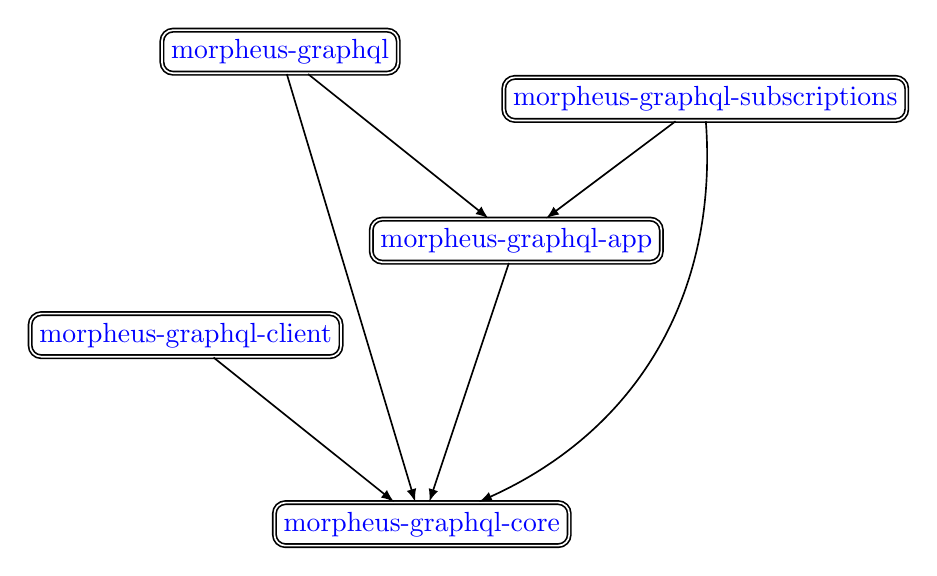
\begin{tikzpicture}[
        scale=.6,
        auto=left,
        -latex ,
        auto ,
        node distance =2 cm and 2cm ,
        % on grid ,
        semithick ,
        package/.style ={ fill=red!20,draw,double,rounded corners ,top color =white ,draw , text=blue , minimum width =1 cm},
    ] 
    \node[package] (core) at (10,0) {morpheus-graphql-core};
    \node[package] (client) at (5,4)  {morpheus-graphql-client};
    \node[package] (app) at (12,6)  {morpheus-graphql-app};
    \node[package] (server) at (7,10)  {morpheus-graphql};
    \node[package] (subs) at (16,9) {morpheus-graphql-subscriptions};
  
    \path (client) edge (core);
    \path (app)  edge (core);
    \path (server)  edge  (core);
    \path (server)  edge  (app);
    \path (subs)  edge  (app);
    \path 
        (subs) 
            edge [bend left =35] 
        (core);  

\end{tikzpicture}
\end{center}
\end{figure}

